% Компіляція: lualatex -shell-escape main.tex (двічі)
\documentclass[12pt,a4paper]{article}

\usepackage{fontspec}
\usepackage{polyglossia}
\setdefaultlanguage{ukrainian}
\setmainfont{NewComputerModern10}
\setsansfont{Noto Sans}
\setmonofont{Noto Sans Mono}[
  Scale=0.82,
  ItalicFont={Noto Sans Mono},
  ItalicFeatures={FakeSlant=0.2}
]

\usepackage{
  amsmath,
  amssymb,
  array,
  booktabs,
  caption,
  enumitem,
  float,
  geometry,
  graphicx,
  microtype,
  titlesec,
  xcolor
}
\geometry{left=2cm,right=2cm,top=2cm,bottom=2cm}
\setlength{\parindent}{1.25cm}
\setlength{\parskip}{0pt}
\linespread{1.08}

\titleformat{\section}
  {\normalfont\fontsize{14}{16}\selectfont\bfseries}
  {\thesection}{0.6em}{}
\titleformat{\subsection}
  {\normalfont\fontsize{12}{14}\selectfont\bfseries}
  {\thesubsection}{0.6em}{}
\titlespacing*{\section}{0pt}{1.4em}{0.65em}
\titlespacing*{\subsection}{0pt}{1.1em}{0.45em}
\captionsetup{font=small,labelfont=bf,labelsep=endash}
\captionsetup[table]{position=bottom,skip=5pt}

\usepackage[newfloat]{minted}
\SetupFloatingEnvironment{listing}{name=Лістинг}
\setminted{
  fontsize=\scriptsize,
  linenos,
  breaklines,
  breakanywhere,
  frame=single,
  framesep=2mm,
  bgcolor=gray!5,
  tabsize=4
}

\usepackage[
  unicode,
  colorlinks=true,
  linkcolor=black,
  urlcolor=blue,
  pdftitle={ІО-41, Давидчук А. М., Паралельні та розподілені обчислення, Лабораторна робота №1.2},
  pdfauthor={Давидчук Артем Миколайович},
  pdfsubject={Потоки в бібліотеці PThread}
]{hyperref}

\newcommand{\studentName}{Давидчук А. М.}
\newcommand{\studentGroup}{ІО-41}
\newcommand{\recordBook}{4106}
\newcommand{\teacherName}{Корочкін О. В.}
\newcommand{\reportYear}{2026}

\begin{document}

\pagenumbering{gobble}
\begin{titlepage}
  \begin{center}
    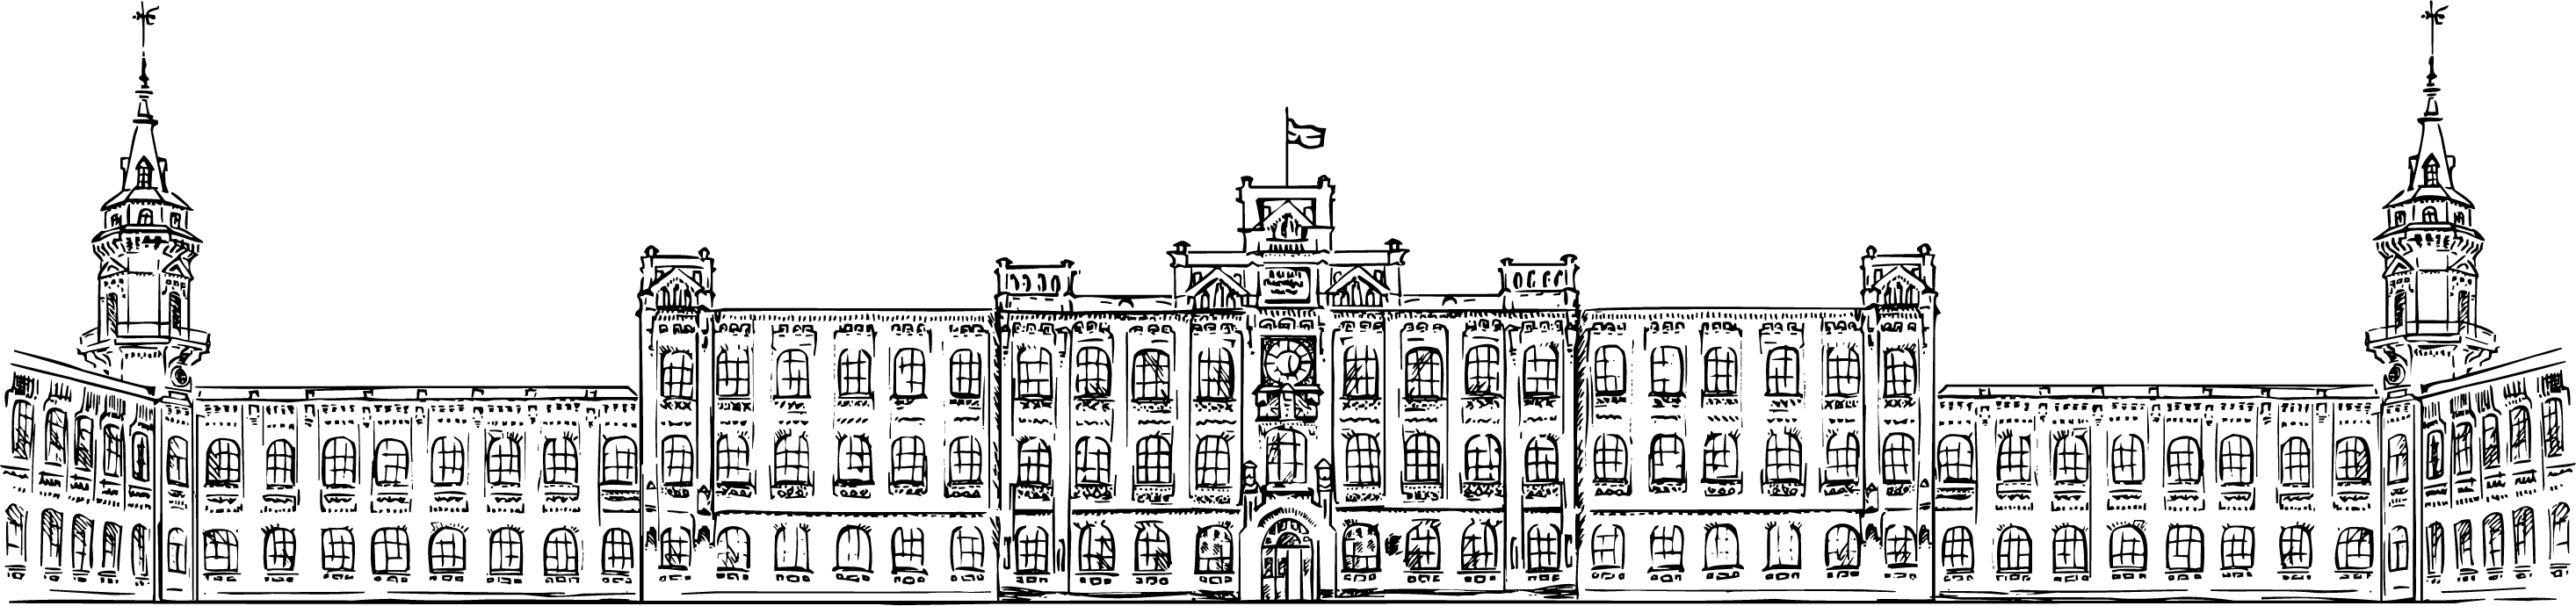
\includegraphics[width=0.7\textwidth]{../../../../../../templates/letterhead.png}
  \end{center}

  \begin{center}
    \large
    Національний технічний університет України\\
    «Київський політехнічний інститут імені Ігоря Сікорського»\\[1em]
    Факультет інформатики та обчислювальної техніки\\
    Кафедра обчислювальної техніки
  \end{center}

  \vfill

  \begin{center}
    \textbf{\LARGE Паралельні та розподілені обчислення}\\[2em]
    \textbf{\Large Лабораторна робота №1.2}\\[0.7em]
    \parbox{0.9\textwidth}{\centering
      «Потоки в бібліотеці PThread»}
  \end{center}

  \vfill

  \begin{flushright}
    \begin{minipage}{0.48\textwidth}
      Виконав: студент 3 курсу ФІОТ,\\
      групи \studentGroup\\
      \textit{\studentName}\\
      Залікова книжка № \recordBook\\
      Номер у списку групи: 6\\[1em]
      Перевірив: \textit{\teacherName}
    \end{minipage}
  \end{flushright}

  \vfill

  \begin{center}Київ --- \reportYear\end{center}
\end{titlepage}

\pagenumbering{arabic}
\tableofcontents
\newpage

\section{Тема та мета роботи}

\noindent
\textbf{Тема:} програмування незалежних потоків засобами бібліотеки
PThread.

\medskip

\noindent
\textbf{Мета:} набути практичних навичок створення, запуску та очікування
потоків у мові C; реалізувати паралельне обчислення незалежних функцій над
векторами й матрицями; дослідити особливості одночасного введення та
виведення; оцінити прискорення програми при використанні одного і трьох
процесорних ядер.

\section{Завдання}

Варіант визначено номером 6 у списку групи. Необхідно створити модуль
\texttt{Data} з операціями лінійної алгебри та три незалежні потоки
\(T_1\), \(T_2\), \(T_3\), які обчислюють такі функції:

\begin{align}
  F_1\ (1.6):\quad MD &= (B\cdot C)\,(MA\cdot ME),
  \label{eq:f1}\\
  F_2\ (2.6):\quad MG &= \operatorname{TRANS}(MK) \cdot (MH\cdot MF),
  \label{eq:f2}\\
  F_3\ (3.6):\quad O &= \operatorname{MAX}(MP\cdot MR) \cdot V.
  \label{eq:f3}
\end{align}

Тут великі латинські літери позначають вектори, подвійні --- квадратні
матриці, \(\operatorname{TRANS}\) --- транспонування, а
\(\operatorname{MAX}\) --- пошук найбільшого елемента матриці.

Розмірність усіх векторів і матриць задається змінною \(N\). Для
\(N=3\) кожен потік має самостійно зчитати одне ціле число і заповнити ним
усі свої початкові дані. Для \(N=1000\) дані мають генеруватися випадково.
Потрібно виміряти час від початку створення потоків до завершення всіх
трьох потоків та визначити прискорення на трьох ядрах порівняно з одним.

\section{Опис програми}

\subsection{Структура програми}

Програму написано мовою C стандарту C11. Для багатопотокового виконання
використано POSIX Threads. Проєкт складається з таких частин:

\begin{itemize}[leftmargin=*,itemsep=0.3em]
  \item \texttt{data.h} --- оголошення типів вектора \texttt{vec\_t},
    квадратної матриці \texttt{sqrmatrix\_t} та операцій над ними;
  \item \texttt{data.c} --- створення і звільнення даних, заповнення одним
    або випадковими значеннями, скалярний добуток, множення матриць,
    множення на скаляр, транспонування та пошук максимуму;
  \item \texttt{main.c} --- функції потоків \texttt{F1}, \texttt{F2},
    \texttt{F3}, введення \(N\), створення потоків та вимірювання часу;
  \item \texttt{CMakeLists.txt} --- опис складання виконуваного файла
    \texttt{lab1} і підключення бібліотеки потоків.
\end{itemize}

Матриця порядку \(N\) зберігається в одновимірному динамічному масиві у
порядку рядків. Елемент з індексами \((i,j)\) розташований за адресою
\texttt{i * N + j}. Результативні операції повертають нові об'єкти, пам'ять
яких звільняється після виведення результату.

\subsection{Алгоритми потоків}

Потоки не використовують спільних математичних даних. Кожен отримує
окремий елемент масиву \texttt{function\_args\_t} зі значеннями \(N\),
режимом заповнення та числом для заповнення.

\begin{table}[H]
  \centering
  \renewcommand{\arraystretch}{1.25}
  \begin{tabular}{|c|p{4.2cm}|p{7.3cm}|}
    \hline
    \textbf{Потік} & \textbf{Вхідні дані} & \textbf{Послідовність обчислень} \\
    \hline
    \(T_1\) & \(B,C,MA,ME\) &
      Обчислити \(s=B\cdot C\), \(M=MA\cdot ME\), потім \(MD=sM\). \\
    \hline
    \(T_2\) & \(MK,MH,MF\) &
      Побудувати \(MK^T\), обчислити \(M=MH\cdot MF\), потім
      \(MG=MK^T M\). \\
    \hline
    \(T_3\) & \(MP,MR,V\) &
      Обчислити \(M=MP\cdot MR\), знайти \(m=\max(M)\), потім
      \(O=mV\). \\
    \hline
  \end{tabular}
  \caption{Локальні дані та алгоритми потоків}
  \label{tab:threads}
\end{table}

Для \(N=3\) функція \texttt{read\_fill\_value} викликається безпосередньо
з відповідної функції потоку. Засоби синхронізації введення і виведення не
використовуються, що дозволяє спостерігати характерні проблеми конкурентної
роботи зі стандартними потоками введення та виведення. Для \(N=1000\)
читання з клавіатури пропускається, а початкові дані заповнюються числами
від 0 до 9.

\subsection{Створення потоків і вимірювання часу}

Головна функція створює потоки викликами \texttt{pthread\_create}, після
чого очікує їх завершення через \texttt{pthread\_join}. Час вимірюється
монотонним годинником \texttt{CLOCK\_MONOTONIC}. Початкова позначка
фіксується безпосередньо перед першим \texttt{pthread\_create}, а кінцева
--- після останнього \texttt{pthread\_join}:

\begin{equation}
  t = (s_2-s_1)+\frac{ns_2-ns_1}{10^9}.
\end{equation}

Отже, вимір охоплює створення потоків, виконання всіх трьох функцій та
очікування їх завершення. Для \(N=3\) до нього також входить час ручного
введення, тому для оцінювання продуктивності використовувалися лише запуски
з \(N=1000\).

\section{Тестування та результати}

\subsection{Перевірка для \texorpdfstring{\(N=3\)}{N=3} і проблема конкурентного введення}

Для контрольного запуску передбачено такі конкретні вхідні дані:

\begin{itemize}[leftmargin=*,itemsep=0.25em]
  \item у потоці \(T_1\) користувач вводить число 1, тому кожний елемент
    векторів \(B,C\) і матриць \(MA,ME\) дорівнює 1;
  \item у потоці \(T_2\) користувач вводить число 2, тому кожний елемент
    матриць \(MK,MH,MF\) дорівнює 2;
  \item у потоці \(T_3\) користувач вводить число 3, тому кожний елемент
    матриць \(MP,MR\) і вектора \(V\) дорівнює 3.
\end{itemize}

Для цих вхідних даних аналітична перевірка дає такі результати:

\begin{itemize}[leftmargin=*,itemsep=0.35em]
  \item у \(F_1\): \(B\cdot C=3\), кожний елемент \(MA\cdot ME\)
    дорівнює 3, тому всі елементи \(MD\) дорівнюють 9;
  \item у \(F_2\): кожний елемент \(MH\cdot MF\) дорівнює 12, тому
    всі елементи \(MG\) дорівнюють \(3\cdot2\cdot12=72\);
  \item у \(F_3\): всі елементи \(MP\cdot MR\) дорівнюють 27,
    отже \(O=27V=(81,81,81)\).
\end{itemize}

Отже, за умови коректної передачі значень відповідним потокам очікуються
матриці зі значеннями 9 і 72 та вектор зі значеннями 81. Проте фактичний
інтерактивний запуск без засобів синхронізації дав іншу картину:

\begin{listing}[H]
\inputminted[firstline=1,lastline=4,fontsize=\footnotesize]{text}{out.txt}
\caption{Повний термінальний вивід проблемного запуску з \(N=3\)}
\end{listing}

У зафіксованому запуску три запрошення надруковано в одному рядку, а
повідомлень з результатами та \texttt{Completed} немає, тобто запуск не
завершився штатно. Причиною є відсутність прикладного протоколу доступу до
спільних потоків \texttt{stdin} і \texttt{stdout}. Після створення потоків
планувальник може передати керування будь-якому з них, тому послідовність
викликів \texttt{printf} і \texttt{scanf} заздалегідь невідома.

Стандартна бібліотека конкретної системи може внутрішньо захищати одну
операцію \texttt{scanf} блокуванням об'єкта \texttt{FILE}, але це не задає
потрібного програмі порядку \(T_1\to T_2\to T_3\). Перший введений символ
отримає той потік, який фактично першим захопив \texttt{stdin}, а не
обов'язково \(T_1\). Інші потоки в цей час очікують доступу до потоку або
наступних чисел. Через це користувач бачить одразу кілька запрошень, не може
надійно визначити адресата введеного числа, а програма може виглядати
завислою.

Аналогічна проблема виникає під час виведення: одна матриця друкується
кількома викликами \texttt{printf}, між якими планувальник може запустити
інший потік. У результаті рядки матриць і службові повідомлення здатні
перемішуватися. Крім того, для \(N=3\) виміряний час охоплює очікування
клавіатурного введення, тому не характеризує швидкість обчислень. Типовим
розв'язанням було б серіалізувати введення mutex-ом або виконати його до
створення потоків, однак у цій роботі синхронізація навмисно не
застосовується, щоб продемонструвати проблему.

\subsection{Дослідження для \texorpdfstring{\(N=1000\)}{N=1000}}

Програму зібрано за допомогою CMake і компілятора GCC 16.2.1. Вимірювання
виконано в Linux на ноутбуці з процесором AMD Ryzen 7 7730U, який надає 16
логічних процесорів. Для обмеження спорідненості процесу використано
\texttt{taskset}: ключ \texttt{-c 0} для одного ядра та \texttt{-c 0-2}
для трьох ядер. У кожному режимі виконано три запуски.

Нижче без скорочень наведено термінальний журнал усіх шести запусків із
іменем користувача, командою запуску, порядком завершення функцій і часом,
який вивела сама програма. Отже, числа в підсумковій таблиці взято
безпосередньо з фактичного виконання, а не отримано розрахунково.

\begin{listing}[H]
\inputminted[firstline=6,lastline=34]{text}{out.txt}
\caption{Повний журнал трьох запусків на одному ядрі}
\label{lst:one-core}
\end{listing}

\begin{listing}[H]
\inputminted[firstline=36,lastline=64,fontsize=\scriptsize]{text}{out.txt}
\caption{Повний журнал трьох запусків на трьох ядрах}
\label{lst:three-cores}
\end{listing}

Результати з лістингів~\ref{lst:one-core} і~\ref{lst:three-cores}
узагальнено в табл.~\ref{tab:timing}.

\begin{table}[H]
  \centering
  \renewcommand{\arraystretch}{1.2}
  \begin{tabular}{|c|c|c|}
    \hline
    \textbf{Номер запуску} & \textbf{Одне ядро, с} & \textbf{Три ядра, с} \\
    \hline
    1 & 11{,}330594 & 5{,}355084 \\ \hline
    2 & 11{,}162718 & 5{,}480508 \\ \hline
    3 & 10{,}868024 & 6{,}432790 \\ \hline
    Середнє & 11{,}120445 & 5{,}756127 \\ \hline
  \end{tabular}
  \caption{Час виконання програми для \(N=1000\)}
  \label{tab:timing}
\end{table}

Коефіцієнт прискорення обчислено за середніми значеннями:

\begin{equation}
  K_p=\frac{t_1}{t_3}=\frac{11{,}120445}{5{,}756127}=1{,}932.
\end{equation}

Ефективність використання трьох ядер становить

\begin{equation}
  E_3=\frac{K_p}{3}\cdot100\%\approx64{,}4\%.
\end{equation}

Завантаження процесорних ядер під час контрольних запусків показано на
рис.~\ref{fig:cpu-load}. В однопроцесорному режимі ядро C0 завантажене на
100\%, тоді як інші ядра майже не використовуються. Після дозволу ядер
C0--C2 усі три досягають 100\% навантаження під час паралельного виконання.

\begin{figure}[H]
  \centering
  \begin{minipage}{0.49\textwidth}
    \centering
    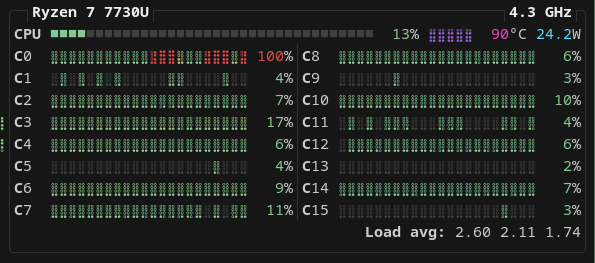
\includegraphics[width=\textwidth]{0cores.png}\\[-0.2em]
    \small а) одне ядро
  \end{minipage}\hfill
  \begin{minipage}{0.49\textwidth}
    \centering
    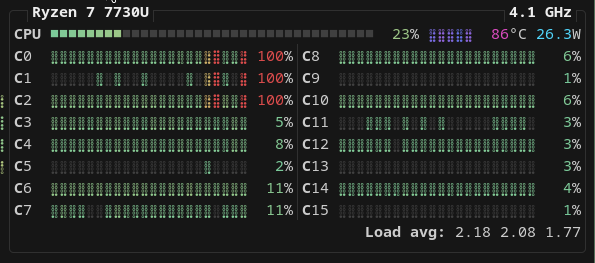
\includegraphics[width=\textwidth]{0-2cores.png}\\[-0.2em]
    \small б) три ядра
  \end{minipage}
  \caption{Завантаження процесора для \(N=1000\)}
  \label{fig:cpu-load}
\end{figure}

Прискорення менше теоретичного максимуму 3 через різний обсяг роботи
потоків: \(F_2\) виконує два множення матриць, тоді як \(F_1\) і \(F_3\)
--- по одному. Після завершення коротших потоків частина ядер простоює,
очікуючи \(T_2\). Додатковий вплив мають створення потоків, виділення
пам'яті, генерація початкових даних та конкуренція за кеш і пропускну
здатність пам'яті.

\section{Висновки}

У лабораторній роботі реалізовано модуль операцій над динамічними векторами
та квадратними матрицями й три незалежні функції варіанта 6. Кожна функція
виконується окремим потоком PThread, має власні локальні дані, самостійно
вводить значення для \(N=3\), обчислює й виводить результат. Аналітична
перевірка показала, що для значень 1, 2 і 3 очікуються матриці зі значеннями
9 і 72 та вектор зі значеннями 81.

Експеримент без синхронізації введення і виведення показав, що порядок
роботи потоків не визначений. У фактичному запуску всі три запрошення
об'єдналися в один рядок, результати не були отримані, а виконання не
завершилося штатно. Відповідність введених чисел потокам визначається
порядком, у якому вони отримують доступ до \texttt{stdin}, тому вона не
гарантує послідовності \(T_1,T_2,T_3\). Виведення також може
перемішуватися між окремими викликами \texttt{printf}. Це демонструє
необхідність узгодження доступу до спільного введення і виведення; за умовою
цієї роботи mutex та інші засоби синхронізації не застосовувалися.

Для \(N=1000\) середній час на одному ядрі становив 11{,}120445 с, а на
трьох --- 5{,}756127 с. Отримане прискорення 1{,}932 підтверджує користь
паралельного виконання незалежних функцій. Неповна ефективність пояснюється
нерівномірним навантаженням потоків і накладними витратами пам'яті та
керування потоками.

\clearpage
\appendix
\section{Лістинг програми}

\subsection{Головний модуль \texttt{main.c}}
\inputminted{c}{../src/main.c}

\subsection{Заголовний файл \texttt{data.h}}
\inputminted{c}{../src/include/data.h}

\subsection{Реалізація модуля \texttt{data.c}}
\inputminted{c}{../src/include/data.c}

\subsection{Файл складання \texttt{CMakeLists.txt}}
\inputminted{cmake}{../src/CMakeLists.txt}

\end{document}
